\newpage

\section{Detekcja oczu} \label{section:eye_detection}

W tej pracy dyplomowej dużą role odgrywają oczy i ich wpływ na sterowanie aplikacją. Z tego powodu musiała zostać określona i zaimplementowana skuteczna metoda ich detekcji.



\subsection{Algorytmy detekcji oczu}

Na potrzeby tego etapu zostały zastosowane dwie metody opierające się na algorytmach opisanych wcześniej - klasyfikatory kaskadowe oraz facemarki.

\subsubsection{Klasyfikator kaskadowy Haar}

Metody detekcji oparte na klasyfikatorach kaskadowych zostały opisane w rozdz. \hyperref[{section:face_casacde_classifier}]{\textit{\ref{section:face_casacde_classifier}}}. Do detekcji oczu z użyciem tego algorytmu zostanie wykorzystany model autorstwa Shameem Hameed \cite{eye_haar_model}.

\subsubsection{Facemarki}

Opisane w rozdz. \hyperref[section:landmarks]{\ref{section:landmarks}} facemarki nanoszą punkty charakterystyczne na obraz twarzy. Znajdują się one m.in. wokół oczu. Fakt ten można wykorzystać do detekcji ich obszaru. Celem uzyskania takiego efektu należy wyznaczyć prostokąt, który będzie otaczał wszystkie sześć facemarków danego oka. \cite{detect_eye_facemarks}
\par
Przykład takiego działania widoczny jest na rysunku \ref{fig:facemarki_to_detect_eyes}.

\begin{figure}[!h]
    \begin{center}
        \subfigure[Facemarki wokół oka]{\label{fig:facemarki_to_detect_eyes_no_rect}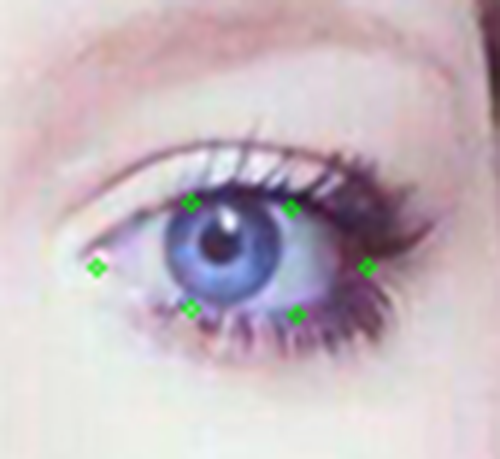
\includegraphics[scale=0.25]{img/eye_section/eye_facemarks.png}}
        \hspace{8mm}
        \subfigure[Naniesiony prostokąt otaczający facemarki wokół oka]{\label{fig:facemarki_to_detect_eyes_rect}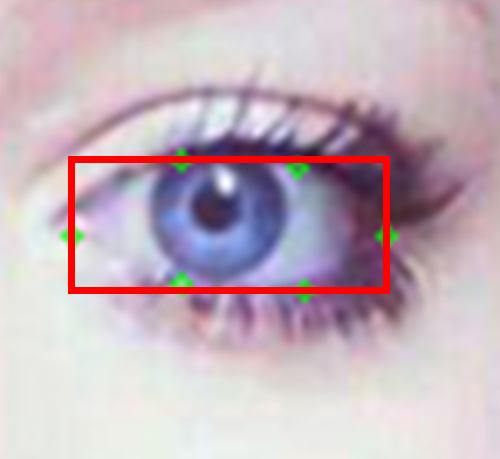
\includegraphics[scale=0.25]{img/eye_section/eye_facemarks_rect.png}}
    \end{center}
    \caption{Wykorzystanie facemarków do detekcji obszaru oczu}
    \label{fig:facemarki_to_detect_eyes}
\end{figure}

Wykorzystywany jest tu też wskaźnik \textit{EAR} (patrz rozdz. \hyperref[{section:EARsection}]{\textit{\ref{section:EARsection}. EAR - Eye Aspect Ratio}}) do wykrycia czy oko jest zamknięte czy otwarte.
\par
Skuteczność tej metody zależy od dokładności algorytmu odwzorowującego facemarki. Ewentualne niedoskonałości można niwelować zwiększając wielkość prostokąta o pewną tolerancję. Taki współczynnik w projekcie został testowo ustalony, a wyniki i wartości parametrów opisane w rozdz. \hyperref[{section:facemark_eye_size}]{\textit{\ref{section:facemark_eye_size}}}.



\subsection{Filtrowanie wyników metody Haar}

Ze względu, że algorytmu Haar może zwracać większą ilość prawdopodobnych obszarów, w których spodziewa się on wykryć pożądany obiekt, wprowadziłem filtrowanie wyników detekcji oczu. \\
Algorytm filtrowania składa się z dwóch etapów:

\begin{itemize}
    \item Podzielenie wykrytych obszarów na dwie grupy - na lewą i prawą stronę twarzy
    \item W obu grupach wybranie największego obszaru
\end{itemize}


Dodatkowo pozwoliło to na łatwe zidentyfikowanie który obszar to które oko i ich posortowanie.
\par
Przykładowy rezultat takiego filtrowania pokazany jest na \hyperref[{fig:eye_filter}]{\textit{rysunku \ref{fig:eye_filter}}}. 


\begin{figure}[!h]
    \begin{center}
        \subfigure[Przed filtrowaniem]{\label{fig:eye_filter_before}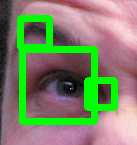
\includegraphics[scale=1.0]{img/eye_section/eye_filter_before.png}}
        \hspace{8mm}
        \subfigure[Po filtrowaniu]{\label{fig:eye_filter_after}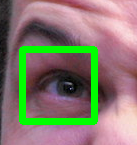
\includegraphics[scale=1.0]{img/eye_section/eye_filter_after.png}}
    \end{center}
    \caption{Efekt filtrowania obszarów detekcji oczu}
    \label{fig:eye_filter}
\end{figure}

\subsection{Obcięcie obszaru detekcji dla metody Haar}

Dla metody opartej na Haar zdecydowałem się dodatkowo zawęzić płaszczyznę przeszukiwań na niecałą twarz, celem uzyskania wyników lepszych niż bez takiego zmniejszenia. 
\par
Ustalenie jaki obszar da najlepszy rezultat odbyło się przez testowe sprawdzanie kombinacji trzech parametrów oznaczających jaka część wykrytej twarzy zostaje obcięta z poszczególnej strony. Mogą one przyjmować wartości w następujących przedziałach:

\begin{itemize}
    \item Góra: $[0.0,$ $0.02]$
    \item Dół: $[0.2,$ $0.6]$
    \item Boki: $[0.0,$ $0.02]$
\end{itemize}

Każdy parametr mógł osiągać wartości będące wielokrotnością $0.05$ w poszczególnych przedziałach.

\par

Ze względu na dużą ilość kombinacji ($225$) nie zostaną podane wyniki, a jedynie wybrana najlepsza kombinacja:
\begin{itemize}
    \item Góra: $0.05$
    \item Dół: $0.3$
    \item Boki: $0.0$
\end{itemize}

Algorytm Haar uzyskał lepszą skuteczność detekcji wykorzystując dodatkowe obcięcie niż bez niego:

\begin{table}[!h]

\centering
\caption{Skuteczność algorytmu detekcji oczu Haar z dodatkowym obcięciem i bez}
\label{tab:eye_haar_crop_result}
\resizebox{\textwidth}{!}{%
\begin{tabular}{|c|c|c|c|c|c|c|}
\hline
 &
  \textbf{\begin{tabular}[c]{@{}c@{}}Prawidłowe\\ detekcje\end{tabular}} &
  \textbf{\begin{tabular}[c]{@{}c@{}}Perfekcyjne\\ detekcje\end{tabular}} &
  \textbf{\begin{tabular}[c]{@{}c@{}}Częściowo\\ dobre\\ detekcje\end{tabular}} &
  \textbf{\begin{tabular}[c]{@{}c@{}}Złe\\ detekcje\end{tabular}} &
  \textbf{\begin{tabular}[c]{@{}c@{}}Niewykryte\\  oczy otwarte\end{tabular}}  &
 \textbf{\begin{tabular}[c]{@{}c@{}}Niewykryte\\  oczy zamknięte \end{tabular}} \\ \hline \hline
\textbf{Haar bez obcięcia} &
  124 &
  85 &
  39 &
  34 &
  8 &
  32  \\ \hline

\textbf{Haar z obcięciem} &
  133 &
  95 &
  38 &
  23 &
  9 &
  11  \\ \hline
  
  \hline
\end{tabular}%
}
\end{table}

Przykład takiego obcięcia z wybranymi parametrami widoczny jest na \hyperref[{fig:eye_crop}]{\textit{rysunku \ref{fig:eye_crop}}}.

\begin{figure}[!h]
    \begin{center}
        \subfigure[Wykryty obszar twarzy]{\label{fig:eye_crop_before}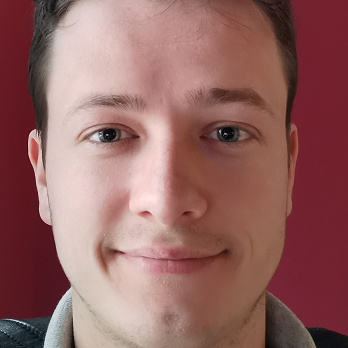
\includegraphics[scale=0.6]{img/eye_section/eye_cropped_face.png}}
        \hspace{8mm}
        \subfigure[Obszar po obcięciu]{\label{fig:eye_crop_after}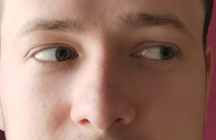
\includegraphics[scale=0.6]{img/eye_section/eye_cropped_eyes.png}}
    \end{center}
    \caption{Obcięcie obszaru detekcji oczu zgodnie z dobranymi wcześniej parametrami}
    \label{fig:eye_crop}
\end{figure}

Wprowadzenie takiej modyfikacji pozwoliło odrzucić część błędnie ustalanych obszarów, szczególnie w dolnej części twarzy. Przykład poprawionej detekcji oczu dzięki temu zabiegowi widoczny jest na rysunku \ref{fig:eye_detect_crop}

\begin{figure}[!h]
    \begin{center}
        \subfigure[Wykrywanie oczu bez dodatkowego obcięcia obszaru]{\label{fig:eye_detect_crop_before}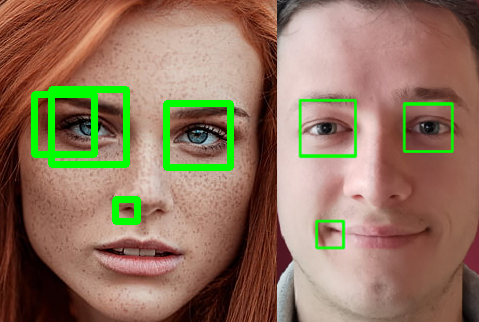
\includegraphics[scale=0.45]{img/eye_section/eye_detect_before_crop_1.png}}
        \hspace{8mm}
        \subfigure[Wykrywanie oczu z dodatkowym obcięciem obszaru]{\label{fig:eye_detect_crop_after}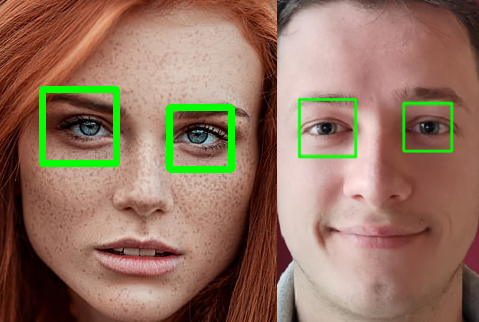
\includegraphics[scale=0.45]{img/eye_section/eye_detect_after_crop_1.png}}
    \end{center}
    \caption{Odrzucenie błędnych rezultatów detekcji oczu po dodatkowym obcięciu obszaru. Źródło pierwszego zdj.:\cite{readheadPortrait2}}
    \label{fig:eye_detect_crop}
\end{figure}


\subsection{Dostosowanie wielkości obszaru facemarków oczu} \label{section:facemark_eye_size}

Dla metody opartej o punkty charakterystyczne twarzy zdecydowałem się dodać pewną tolerancję do obszaru wynikającego jedynie z połączenia tych punktów.
\par
Ustalenie jakie zwiększenie zwracanego regionu da najlepsze rezultaty detekcji oczu odbyło się przez testowe sprawdzenie kombinacji trzech parametrów, które oznaczały wielkość tolerancji z danej strony. W teści przyjmowały one następujące wartości

\begin{itemize}
    \item Góra: z przedziału [0.0, 1.0], będące wielokrotnością $0.1$
    \item Dół: z przedziału [0.0, 1.0], będące wielokrotnością $0.1$
    \item Boki: z przedziału [0.0, 0.5], będące wielokrotnością $0.05$
\end{itemize}

\par

Ze względu na dużą ilość kombinacji ($1331$) nie zostaną podane wyniki, a jedynie wybrana najlepsza kombinacja:
\begin{itemize}
    \item Góra: $0.7$
    \item Dół: $0.5$
    \item Boki: $0.2$
\end{itemize}


\begin{table}[!h]
\label{tab:eye_facemark_size_result}
\centering
\caption{Skuteczność algorytmu detekcji oczu wykorzystując facemarki z dodatkowym zwiększeniem obszaru i bez}
\resizebox{\textwidth}{!}{%
\begin{tabular}{|c|c|c|c|c|c|c|}
\hline
 &
  \textbf{\begin{tabular}[c]{@{}c@{}}Prawidłowe\\ detekcje\end{tabular}} &
  \textbf{\begin{tabular}[c]{@{}c@{}}Perfekcyjne\\ detekcje\end{tabular}} &
  \textbf{\begin{tabular}[c]{@{}c@{}}Częściowo\\ dobre\\ detekcje\end{tabular}} &
  \textbf{\begin{tabular}[c]{@{}c@{}}Złe\\ detekcje\end{tabular}} &
  \textbf{\begin{tabular}[c]{@{}c@{}}Niewykryte\\  oczy otwarte\end{tabular}}  &
 \textbf{\begin{tabular}[c]{@{}c@{}}Niewykryte\\  oczy zamknięte \end{tabular}} \\ \hline \hline
\textbf{\begin{tabular}[c]{@{}c@{}}Facemarki oczu \\ bez zwiększenia obszaru\end{tabular}} &
  142 &
  17 &
  125 &
  14 &
  6 &
  6  \\ \hline

\textbf{\begin{tabular}[c]{@{}c@{}}Facemarki oczu \\ ze zwiększeniem obszaru\end{tabular}} &
  144 &
  142 &
  2 &
  12 &
  6 &
  6  \\ \hline
  
  \hline
\end{tabular}%
}
\end{table}

Zmiany wielkości zwracanego obszaru oczu nie zwiększył znacząco liczby dobrych detekcji. Natomiast największy zysk widoczny jest w perfekcyjnych detekcjach. Dzięki takiemu dostosowaniu udało się osiągnąć prawie $100\%$ wskaźnik perfekcyjnych względem prawidłowych detekcji. Pozwoli to uzyskać lepiej wykryty obszar oczu, co może mieć przełożenie na skuteczność detekcji źrenic.